\documentclass[11pt]{article}
\usepackage[breaklinks=true]{hyperref}
\usepackage{color}
\usepackage{amsmath,amssymb,amsthm}
\usepackage{natbib}
\usepackage{array}
\usepackage{booktabs, multicol, multirow}
\usepackage[nohead, margin=1in]{geometry}
\usepackage[singlespacing]{setspace}
\usepackage{graphicx}


\newtheorem{theorem}{Theorem}[section]
\newtheorem{lemma}[theorem]{Lemma}
\newtheorem{assumption}{Assumption}

\newcommand{\beq}{\begin{equation}}
\newcommand{\eeq}{\end{equation}}
\newcommand{\bit}{\begin{itemize}}
\newcommand{\eit}{\end{itemize}}

\newcommand{\todo}[1]{{\color{red}{TO DO: \sc #1}}}

\newcommand{\reals}{\mathbb{R}}
\newcommand{\integers}{\mathbb{Z}}
\newcommand{\naturals}{\mathbb{N}}
\newcommand{\rationals}{\mathbb{Q}}

\newcommand{\ind}{\mathbb{I}} % Indicator function
\newcommand{\pr}{\mathbb{P}} % Generic probability
\newcommand{\ex}{\mathbb{E}} % Generic expectation
\newcommand{\var}{\textrm{Var}}
\newcommand{\cov}{\textrm{Cov}}

\newcommand{\normal}{N} % for normal distribution (can probably skip this)
\newcommand{\eps}{\varepsilon}
\newcommand\independent{\protect\mathpalette{\protect\independenT}{\perp}}
\def\independenT#1#2{\mathrel{\rlap{$#1#2$}\mkern2mu{#1#2}}}
\newcommand{\argmax}{\textrm{argmax}}
\newcommand{\argmin}{\textrm{argmin}}
\renewcommand{\baselinestretch}{1.5}

\title{A Comparison of Parametric and Permutation Tests for Regression Analysis of Randomized Control Trials}
\author{Kellie Ottoboni \\
Department of Statistics; Berkeley Institute for Data Science\\
University of California, Berkeley\\ [.2in]
Luigi Salmaso\\
Department of Management and Engineering \\
University of Padova \\ [.2in]
Fraser Lewis \\
RB
}\date{Draft \today}
\begin{document}
\maketitle

\newpage

\begin{abstract}
\noindent\textbf{Background:}
In clinical trials, the standard analysis of the effectiveness of one treatment over another is a parametric analysis of covariance (ANCOVA), a method based on linear regression which relies on uncheckable and ostensibly implausible assumptions such as constant treatment effects across groups, normality of errors, and homoskedasticity.
The decision of the effectiveness of the treatment is based upon a single p-value from this hypothesis test, which may not be valid if the assumptions are not met.
One would like to run some sort of robustness check, an additional test or something, whose results can call into question or give evidence in favor of the results from the ANCOVA.

\noindent\textbf{Methods:}
Permutation tests present such an opportunity: they require only minimal assumptions which are often guaranteed by the randomization that was conducted.
In contrast to parametric tests, which rely up on stringent assumptions to obtain null distributions with a simple closed form, permutation tests use the assumption of exchangeability or randomization to construct approximate null distributions by simulation, yielding (approximately) exact tests.
In order to mimic the ANCOVA that is typically done, we compare several permutation tests based on linear models, which enable one to control for pretreatment covariates and nuisance variables.

\noindent\textbf{Results:}
We present simulations showing that the permutation methods maintain power comparable to the ANCOVA in randomized trials.
We illustrate the use of permutation tests alongside the parametric ANCOVA using data from a clinical trial across eight sites with different numbers of patients.

\noindent\textbf{Conclusions:}
These results suggest that the parametric ANCOVA and linear model permutation tests perform similarly, even when the more stringent assumptions for the parametric test are not met.


\end{abstract}

% keywords: permutation test, linear model, ANOVA
\newpage

\section{Background}
% The Background section should explain the background to the study, its aims, a summary of the existing literature and why this study was necessary or its contribution to the field.
A hypothesis test is a statistical method for determining whether observed data is consistent with a hypothesis about the process that generated the data.
Medical trials use hypothesis testing to assess the evidence that a treatment has an effect on one or more clinically relevant outcomes.
The simplest version of this experiment, which involves randomly assigning treatment to a fixed number of individuals in a group and measuring a single outcome, has been studied for nearly a century (see \citet{fisher_design_1935} and \citet{neyman_application_1923} for early references).
One can conduct hypothesis tests and construct confidence intervals for the estimated treatment effect
by exploiting the fact that the difference in average outcomes between the treatment and control groups is asymptotically normal with a variance that can be estimated from the data.

Randomized experiments in the real world are rarely this simple:
individuals are heterogeneous with respect to pretreatment covariates,
they may not take the treatment they are assigned or may drop out of the study,
and an individual's assignment to treatment may affect others' outcomes.
Techniques have been developed to deal with each of these issues.
In this paper, we focus on the first.

Random assignment of treatment ensures that on average, across all possible randomizations, pretreatment covariates are balanced between treatment groups.
However, in any particular randomization that is realized, there may be imbalances.
If these covariates are predictive of the outcome, then even when there is no effect of treatment, differences in outcomes between treatment groups may appear.
Controlling for such baseline covariates can reduce the variability of estimated treatment effects and yield more powerful hypothesis tests.

Another method for controlling for baseline covariates is stratification:
individuals are divided into groups based on levels of some covariate.
A common stratification variable in clinical experiments is location:
individuals often come from many sites because it is difficult to recruit a sufficient number of participants at one doctor's office or hospital.
Treatments are randomly assigned  \textit{within strata} to guarantee that the stratum variable is balanced between treatment groups.
As with other pretreatment covariates, outcomes may vary across strata due to factors unrelated to individuals.
Controlling for stratum can have the same beneficial effects as controlling for other pretreatment covariates.

\todo{not happy with this paragraph}
The most common way to control for covariates is linear regression.
The premise is to project the outcomes onto a linear plane which describes the contribution of each covariate to determining the outcome.
The coefficient of any particular variable answers the question, if we were to hold fixed all other covariates and increase this variable by one unit, how much would the outcome change?
This model posits a linear relationship between covariates, treatment, and outcome; if the true relationship is not linear, then it is unclear what such a regression is estimating.
However, if one knows all covariates related to the outcome and fits a fully saturated linear model (including all covariates and their interactions), the coefficient for the treatment is an asymptotically consistent estimate of the average treatment effect (\cite{lin_agnostic_2013}).
When controlling for strata, such as location, it is standard to use analysis of covariance (ANCOVA), a particular case of linear regression which allows each stratum to have its own mean outcome level.
This amounts to choosing the plane of best fit for the data, allowing each stratum to have a different intercept but enforcing that the slope is the same for each.

Hypothesis testing of estimated coefficients requires even stronger assumptions than linearity, such as normally distributed and homoskedastic errors.
When this holds, the distribution of a coefficient scaled by its estimated variance, has a $t$-distribution.
Thus, a hypothesis test for a treatment effect amounts to a hypothesis test of the coefficient for treatment in the linear model, and can be evaluated analytically and quickly.
However, these assumptions are clearly violated in many cases:
when the data are discrete or ordinal, when the treatment has a differential effect across strata, and when measurement error sizes differ across strata.

An alternative approach is permutation testing.
Deliberate randomization induces a distribution for any test statistic under the null hypothesis that treatment has no effect on the outcome,
because the randomization scheme provides information about all possible ways that treatment may have been assigned 
and the null hypothesis tells us what each individual's response would be regardless of the assignment (namely, it would be the same).
Instead of deciding how ``extreme'' the observed test statistic is relative to a parametric reference distribution, such as Student's $t$ or the Gaussian, one judges it against this randomization distribution.
Such a test is exact, meaning that it controls the type I error rate at the pre-specified level, even in finite samples, whereas parametric hypothesis tests based on asymptotic approximations do not always guarantee good finite sample properties.
In the past, parametric tests were necessary because asymptotic approximations were the only computationally feasible way to estimate distributions. 
Now, computational power is no longer a barrier to finding exact (or exact to pre-specified precision) randomization distributions.
In most cases, a randomization test is preferable to a parametric one:
``[a] corresponding parametric test is valid only to the extent that it results in the same statistical decision [as the randomization test]'' (\cite{bradley_distribution_1968}).

\todo{ lit review: 
\bit 
\item cite the vickers paper
\item what else have people done comparing linear models to permutation/nonparametric tests?
\eit
}

In this paper, we review ANCOVA and its permutation counterparts, comparing their performance in different scenarios, and illustrating their application with a clinical dataset.
We find in simulations that even when assumptions are not satisfied, the parametric and permutation tests have comparable power to detect a treatment effect.
We apply each of the methods to data from a clinical trial seeking to compare the performance of two treatments for gastroesophageal reflux disease (GERD).
We conclude by discussing implications of these results for practitioners.

\section{Methods}
% The methods section should include:

%the aim, design and setting of the study
%the characteristics of participants or description of materials
%a clear description of all processes, interventions and comparisons. Generic drug names should generally be used. When proprietary brands are used in research, include the brand names in parentheses
%the type of statistical analysis used, including a power calculation if appropriate

\subsection{Problem and notation}
Suppose we randomly assign two treatments to a group of individuals
Let $Z$ be treatment assignment, 0 or 1, and we are interested in comparing the relative effectiveness of treatment 1 to treatment 0.
$Y$ is the outcome of interest observed for all individuals.
$X$ is a pretreatment covariate that we observe and is related to the outcome (may or may not be causal).  
Without loss of generality, we suppose that $X$ is univariate, but we could easily extend all of these results to multivariate $X$.

Suppose there is another nuisance variable $\mathcal{J}$. 
$\mathcal{J}$ is a pretreatment variable used to stratify individuals. 
There may be some unobservable heterogeneity in outcomes across levels of $\mathcal{J}$.

We observe $\{Y_{ij}(Z_{ij}), Z_{ij}, X_{ij}\}$ for units $i = 1, \dots, n_j$, in strata $j = 1, \dots, J$.
All units have two potential outcomes, $Y_{ij}(1)$ and $Y_{ij}(0)$, representing their responses to treatments $1$ and $0$, respectively.
We can never observe both; random assignment of treatment reveals one.

We are interested in the differences in potential outcomes $Y_{ij}(1) - Y_{ij}(0)$.
This difference represents the effect of treatment for individual $i$ in group $j$: it is the difference between what we would have observed under treatment 1 and what we would have observed under treatment $0$.
Depending on the method of analysis one chooses, different functions of these differences will be considered.
Any of these quantities may be of clinical interest; it is a matter of philosophy which one prefers.
A typical problem is to estimate one of these averages.
Instead, we will focus on hypothesis testing.
Below, we outline a few approaches to studying the average treatment effect, explain the assumptions that are necessary, and 

\subsection{Parametric ANCOVA}

The model is

$$Y_{ij} = \alpha_j + \beta X_{ij} + \gamma Z_{ij} + \eps_{ij}$$

where $\alpha_j$ is a fixed effect for stratum $j$, $\beta$ is the coefficient for the pretreatment covariate,
$\gamma$ is the coefficient for treatment,
and $\eps_{ij}$ is an error term.
The parameter of interest is $\gamma$, which represents the average treatment effect in the sample. 
We would like to test the null hypothesis $H_0: \gamma = 0$ against
the two-sided alternative hypothesis $H_1: \gamma \neq 0$.

To carry out hypothesis testing using parametric distributions, we make the following assumptions (\cite{freedman_statistical_2005}):

\begin{enumerate}
\item Linearity: the data $Y$ are related to $X$ and $Z$ linearly
\item Constant slopes: stratum only affects the intercept $\alpha_j$, not the slopes $\beta$
\item IID Errors: the $\eps_{ij}$ are independent and identically distributed with mean $0$ and variance $\sigma^2$
\item Independence: if $X$ is random, $\eps \independent X$
\item Normality: the errors are normally distributed
\end{enumerate}

The coefficients are estimated using least squares.\footnote{
Note, only Assumptions (1) and (2) are needed to guarantee the existence of a solution.
If there is a linear relationship between $X$, $Z$, and stratum, the solution will not be unique.
}
A significance test is done for the estimated coefficient $\hat{\gamma}$, using the $t$-distribution with degrees of freedom equal to the number of observations minus the number of parameters estimated (in this case, $N - J - 2$).
The test statistic is
$$ t = \frac{\hat{\gamma}}{\sqrt{ \hat{\sigma}_{\hat{\gamma}}^2}},$$
where $\hat{\sigma}_{\hat{\gamma}}^2$ is the estimated standard error of $\hat{\gamma}$.\footnote{
$\hat{\sigma}_{\hat{\gamma}}^2$ is estimated by first computing the residual standard error $\hat{\sigma}^2$,
then taking the diagonal element corresponding to the treatment variable in the inverse covariance matrix of covariates.
}

\todo{Add a paragraph about why this might go wrong, perhaps some citations. All depends on estimating the error variance correctly, because $t$ distribution is the ratio of a normal and a chi-square}


The ANCOVA model allows for fixed stratum effects, but they are only additive in the outcome.  
The model does not account for differences in the treatment effect across strata.  
The estimated linear model may not accurately capture details of the true data-generating process.  
If effects are not constant across strata, then the coefficient $\gamma$ may be attenuated towards 0.  
A test of the null hypothesis that $\gamma = 0$ will be valid, but will not reflect the true magnitude of treatment effects among individuals.

\subsection{Stratified permutation test}
Suppose we wish to test the null hypothesis that individual by individual, treatment has no effect.
This is referred to as the ``sharp null'' hypothesis:

$$H_0: Y_{ij}(1) = Y_{ij}(0), i = 1, \dots, n_j, j = 1,\dots, J.$$

Then, which treatment that individual $ij$ received amounts to an arbitrary label.
Once we observe their response under treatment $Z_{ij}$, we know what it would have been under treatment $1-Z_{ij}$; namely, it would have been the same.

If treatment was completely randomized across strata, independently across strata,
then we may condition on the number of individuals who received each treatment within each stratum.
Any assignment of treatments which preserves the number of treated units within each stratum is valid and was just as likely to occur as the randomization that was actually observed.
By using this principle of equal probabilities and by imputing the unobserved potential outcomes under the sharp null hypothesis, we can construct the permutation distribution of any statistic under the null hypothesis.

The most commonly used statistic is the difference in mean outcomes of people who received drug 1 and the mean outcomes of people who received drug 0.  This statistic is readily interpretable (``on average, taking the drug changes the outcome by x amount'') and has nice theoretical properties owing to it being the difference of two sums.
When we want to be sensitive to differences in the magnitude of the effect, the difference in means may not be optimal.  For an extreme example, imagine that there are $n/2$ males and $n/2$ females in the sample, $n/4$ males and females receive each treatment.  Those who receive treatment 0 have an outcome of 0, the males who receive treatment 1 have an outcome of 1, and the females who receive treatment 1 have an outcome of -1.  Then the difference in means between the treatment groups will be $0$, even though the treatment had a positive effect on males and negative effect on females.  This differential effect will be averaged out.
Thus, one may want to stratify the sample according to important confounding variables, then take the difference in means within each stratum separately. 

There is a great degree of freedom in choosing how exactly to construct such a statistic.
Two factors must be decided: how to stratify and how to combine the individual means.
There is a tradeoff in how finely we choose to stratify:
on the one hand, we need all of the strata to be sufficiently large, otherwise they don't contribute any information to the test statistic,
 but on the other hand, we want the strata to capture variation in treatment effects.
\todo{discussion of NPC and cite papers}


\subsection{Permutation tests with the linear model}
We would like to test for a difference in outcomes between two treatments, but control for other covariates that may be predictive of the outcome.
For example, if the outcome is the outcome after receiving treatment, we would like to control for the same variable measured before treatment was administered.
When the outcome is the difference in responses between the second and first weeks, we would just like to control for location.
We will use the approximate permutation test derived by Freedman and Lane (1983) to do so.

Under the sharp null $H_0$, $Z$ has no effect on $Y$.
In other words, the null hypothesis is that $\beta_2 = 0$.
In a randomized experiment such as this, there are two ways we may test this null hypothesis.

\subsubsection{Standard linear model}
We may do a variation on the stratified two-sample test described above.
Instead of using the difference in means as the statistic, we can use the t-statistic for the coefficient on $Z$ in a linear regression.
If treatment was assigned at random within each stratum, then it is guaranteed that $Z$ and $\varepsilon$ are statistically independent, conditional on stratum.
Therefore, we may conduct a test by permuting treatment assignments $Z$ within site, independently across sites, and calculating a test statistic for each such permutation.

\subsubsection{Linear model residuals}

Let's take an alternative view of the problem.
We still write $Y = \beta_0 + \beta_1 X + \beta_2 Z + \varepsilon$.
However, now, we do not treat the $\varepsilon$ as random.
They are simply defined to be the diffence between $Y$ and the data's linear projection onto the plane $\beta_0 + \beta_1 X + \beta_2 Z$.

If the null hypothesis is true, then $\varepsilon = Y - \beta_0 - \beta_1X$.
We may regress $Y$ on $X$ to obtain coefficient estimates $\hat{\beta}_0$ and $\hat{\beta}_1$.
Then we would predict the outcome to be $\hat{Y} = \hat{\beta}_0 + \hat{\beta}_1X$
and we may estimate the errors $\hat{\varepsilon}$ by $Y - \hat{Y}$.
The $\hat{\varepsilon}$ approximate the true errors $\varepsilon$ from the true data-generating process, assuming that the null hypothesis is true and the linear model has a reasonable in-sample fit.
Furthermore, under the null hypothesis, the $\varepsilon$ are independent of $X$ and $Z$. \todo{ this is false. fix}
Therefore, within sites, these estimated $\hat{\varepsilon}$ are approximately exchangeable.
Note that the exchangeability is only approximate, because $\hat{\varepsilon}$ will have some correlation with $X$ due to the finite sample size. \todo{ fix wording}

We construct a permutation distribution using several steps:

\begin{enumerate}
\item Estimate $\hat{\varepsilon}$ by $Y - \hat{\beta}_0 - \hat{\beta}_1 X$, where $\hat{\beta}_0$ and $\hat{\beta}_1$ are obtained by regressing $Y$ on $X$.
\item Construct permuted errors $\hat{\varepsilon}^\pi$ by permuting the $\hat{\varepsilon}$ within sites.
\item Construct permuted responses $Y^\pi = \hat{\beta}_0 + \hat{\beta}_1 X + \hat{\varepsilon}$.
\item Regress $Y^\pi$ on $X$ and $Z$. The test statistic is the $t$-statistic for the coefficient of $Z$.
\end{enumerate}


\subsubsection{Other linear model tests}
It is important to note that the permutation tests described here are only exact in the context of randomized experiments.
In observational studies, they are only approximately exact under the best circumstances.
What's the difference between these two situations?
In randomized experiments, treatment is assigned at random, and is therefore statistically independent of the covariates $X$ and the errors $\varepsilon$.
Conversely, in observational studies, treatment may be associated with $X$ and/or $\varepsilon$, often in a way that is difficult or impossible to model.
Independence, or the weaker condition of exchangeability, is what enables us to construct permutation distributions while holding $X$ fixed.
When exchangeability doesn't hold, it does not make sense to permute $Z$ while holding $X$ fixed, as we cannot disentangle the effect of one over the other.
In order to justify the use of one of these linear model tests for a treatment effect in observational data, one must argue that the object being permuted is uncorrelated with the other variables being held fixed.
This can be done visually using scatterplots and residual plots.
\todo{citations!}

Others have developed approximate permutation tests which use linear regression to adjust for covariates. 
\bit
\item Cite a few here, 
\item explain why Freedman-Lane is best. 
\item Cite some people who have shown by simulation that it works better.
\eit


\section{Results}
\subsection{Simulations}

To compare the performance of these tests, we simulated data coming from a randomized experiment, applied the tests to the data, and compared their empirical power over repeated random treatment assignments and random errors.
We compared the following five tests:
the $t$-statistic from the parametric ANOVA,
a stratified permutation test using the difference in mean outcomes\footnote{ We considered using the difference in means within each stratum, aggregated by taking the sum of their absolute values over stratum. However this would not be ideal for imbalanced designs, which are common in real-world applications, so we did not consider it in the simulations.  See the data analysis for details.}
 (called ``stratified permutation'' in what follows),
a stratified permutation test difference mean differences, taken by subtracting the baseline measure from the outcome (called ``differenced permutation'' in what follows),
a stratified permutation test based on the $t$-statistic from the linear regression of outcome on control variables (called ``LM permutation'' in what follows),
and the Freedman-Lane permutation test.
 

We assume the following linear data-generating process:

$$Y_{ij1} =\beta_0Y_{ij0} + \beta_{j} + \gamma_j Z_{ij} + \varepsilon_{ij}$$

for individuals $i = 1, \dots, n_j$, $j = 1, 2, 3$.
$\beta_0$ is the coefficient for the baseline measurement $Y_{ij0}$, 
$\beta_j$ is the mean effect of being in stratum $j$, 
$Z_{ij}$ is the treatment level, 
$\gamma_j$ is the effect of treatment in stratum $j$, 
and $\varepsilon_{ij}$ is an error term.
Suppose there are three strata with $\beta_1 = 1, \beta_2 = 1.5,$ and $\beta_3 = 2$.
Assume that there are $n_j = 16$ individuals per stratum and treatment assignment is balanced, i.e. 8 people receive each treatment within each stratum.

We use two designs:
\begin{itemize}
\item Constant additive treatment effect: $\gamma_1 = \gamma_2 = \gamma_3 = \gamma$. This is the implicit assumption when doing inference on estimated treatment effects.
\item Treatment effect in a single stratum: $\gamma_1 = \gamma > 0$, $\gamma_2 = \gamma_3 = 0$. This is a constant, additive treatment effect in stratum 1, but no treatment effect in strata 2 and 3. This is a simplistic case of heterogeneous treatment effects.
\end{itemize}

We draw the baseline measurements once and condition on observing $\{ Y_{ij0}\}_{i = 1,\dots,16, j = 1,\dots, 3}$.
Then, for a large number of trials, we randomly assign treatment within strata, generate errors, and construct new outcomes $Y_{ij1}$.
We conduct all five tests on this new data, obtaining a two-sided p-value for each.
The power curves are estimated by computing the proportion of observed p-values less than or equal to $\alpha$, for $\alpha = 0.01, 0.02, \dots, 1$.

In our first set of simulations, we assume that the baseline measurements $Y_{ij0}$ are standard normally distributed and the pairs $(Y_{ij0}, \varepsilon_{ij})$ are independent across $i$ and $j$.
We will assume that $\beta_0 = 1$.
For each of the two simulation designs that vary the treatment effect, we use two distributions of $\varepsilon$.
In the first case, we use $\varepsilon \sim N(0, 1)$ to fit with the parametric ANOVA assumption of normal errors.
In the second case, $\varepsilon$ comes from a $t$ distribution with 2 degrees of freedom so the errors are heavy-tailed.
Thus, there are four total simulation designs.

Figure~\ref{fig:normal_sim_power} shows the estimated power curves in these four designs using a treatment effect of $\gamma = 1$.
The best case is when the errors are Gaussian and the treatment effect is constant across strata, while the worst case is when the errors are heavy-tailed and the treatment effect only appears in one stratum.
\todo{it makes sense that this happens as assumptions are broken in other cases}
A consistent pattern appears in each case: the stratified permutation test has the lowest power, while the other four tests tend to have very similar power.
Table~\ref{tab:normal_power} displays the value of these power curves at level $0.05$.
These numbers show that actually, for $\alpha=0.05$, the discrepancy between the stratified permutation test and the others is not so large when the effect is isolated in a single stratum.
In this case, the permutation test may have more power than the parametric ANOVA at significance levels that are used in practice.


\begin{figure}
\centering
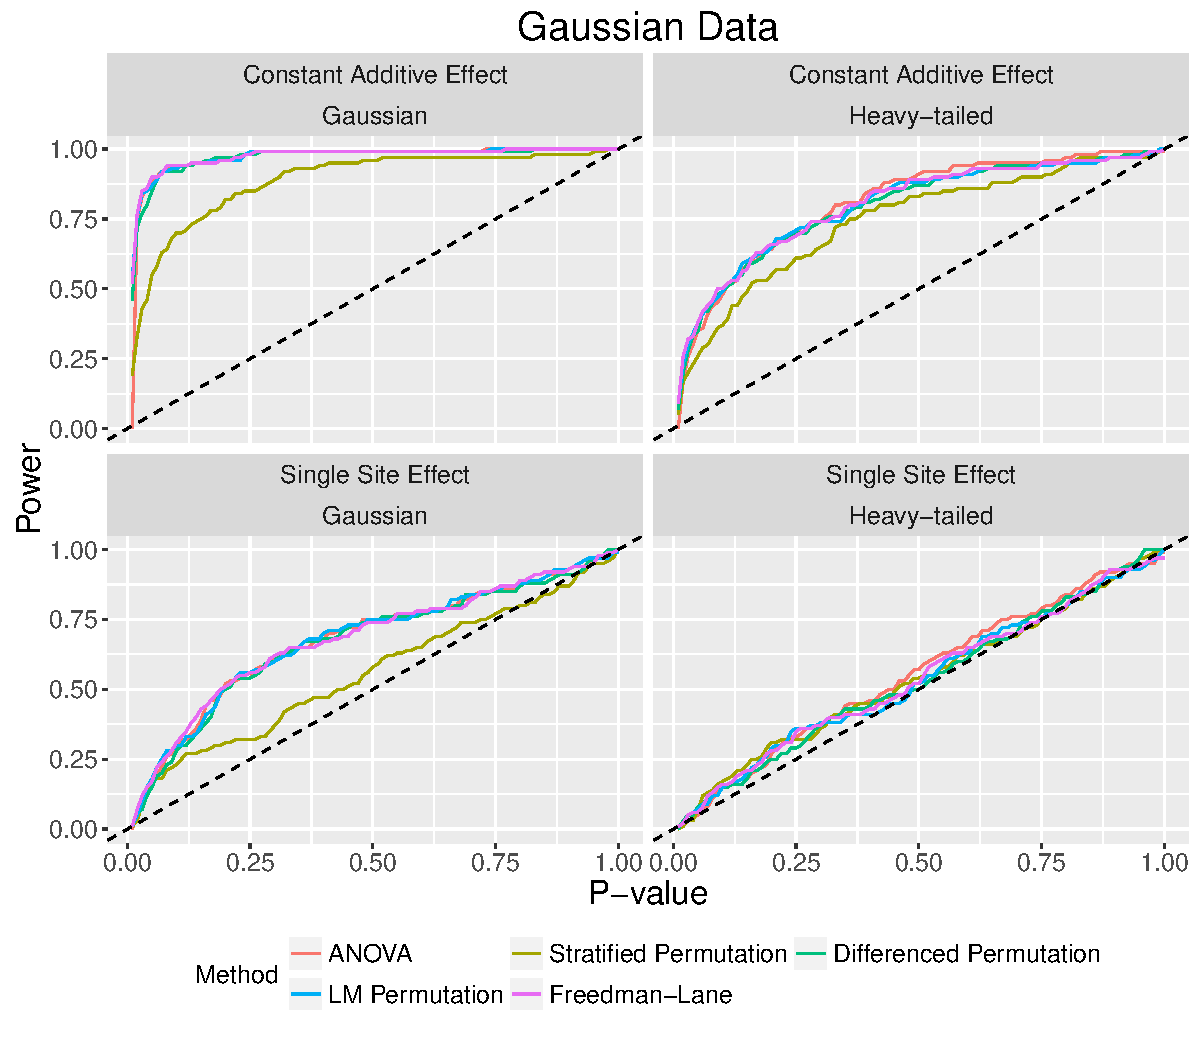
\includegraphics[width = \textwidth]{fig/normal_simulation_power}
\caption{Empirical power curves for the Gaussian simulated data}
\label{fig:normal_sim_power}
\end{figure}
\begin{center}
\begin{table}[ht]
\centering
\begin{tabular}{p{1.15in}|p{0.7in}|p{0.6in}p{0.8in}p{0.8in}p{0.8in}p{0.75in}}
  \hline
Treatment & Errors & ANOVA & Stratified Permutation & Differenced Permutation & LM Permutation & Freedman-Lane \\ 
  \hline
Constant Additive Effect & Gaussian & 0.89 & 0.55 & 0.86 & 0.89 & 0.89 \\ 
  Single Stratum Effect & Gaussian & 0.16 & 0.09 & 0.16 & 0.16 & 0.17 \\ 
  Constant Additive Effect & Heavy-tailed & 0.35 & 0.24 & 0.38 & 0.40 & 0.39 \\ 
  Single Stratum Effect & Heavy-tailed & 0.07 & 0.08 & 0.08 & 0.08 & 0.08 \\ 
   \hline
\end{tabular}
\caption{Empirical power at level $0.05$ for Gaussian simulated data} 
\label{tab:normal_power}
\end{table}

\end{center}

In our second set of simulations, we assume that the baseline measurements $Y_{ij0}$ are discrete and skewed.
This is representative of some survey data, where individuals are asked to rate their experience on a scale from 1 to 10, for instance.
Here, we generate the baseline measures using independent draws from a Poisson distribution with mean 4, and censoring values larger than 10, instead setting them to 10.
We condition on these observed baseline measures once we have generated them once.
Then, for each of the large number of trials, we randomly assign treatment within strata and generate errors taking on values $0.5$ and $-0.5$ with equal probability.
We construct $Y_{ij1}$ using the linear equation above.
However we don't observe $Y_{ij1}$ but instead $\tilde{Y}_{ij1}$, which is defined as 

\begin{displaymath}
   \tilde{Y}_{ij1} = \left\{
     \begin{array}{ll}
       1 & \text{if } \tilde{Y}_{ij1} < 1\\
       10 & \text{if } \tilde{Y}_{ij1} > 10 \\
       \lfloor \tilde{Y}_{ij1} \rfloor & \text{otherwise}
     \end{array}
   \right.
\end{displaymath}

The observed outcomes $\tilde{Y}_{ij1}$ that we test are also discrete.
The assumption of normality is clearly violated here.

In these simulations, we examine the effect of sample size.
First, we consider balanced samples, where each stratum contains 16 individuals, 8 of whom receive one treatment and the other 8 of whom receive the other.
Next, we consider imbalanced samples, where the smallest stratum has only 8 individuals, the next has 16, and the largest has 24.
We again consider the four combinations of treatment effects and sample sizes.
In the case where there is only a non-null treatment effect in one stratum and sample sizes are different, this effect occurs in the smallest stratum.

Figure~\ref{fig:skewed_sim_power} shows the estimated power curves in these four designs using a treatment effect of $\gamma = 0.5$.
When the treatment effect is constant, sample sizes within each stratum don't matter; the power curves look the same up to chance variation.
When the treatment effect only occurs in one stratum, there is a substantial loss in power due to halving the number of individuals in the stratum where the effect is present.
In practice, one does not usually know a priori which individuals will be affected by treatment (otherwise, those unaffected by treatment would be excluded from the study altogether),
so this result suggests using caution when stratifying.
As in the first set of simulations, the stratified permutation test using the raw outcomes has the lowest power of the five tests.
Now, however, the stratified permutation test using the difference between outcome and baseline also has lower power than the three using linear models.
Presumably, this is because the differences are also discrete and lie in a small range of values, so the test statistic does not vary greatly across permutations.
Table~\ref{tab:skewed_power} confirms this: power for the three linear model methods is high when the treatment is constant across strata, and power for all of the methods suffers when the effect is isolated in a single stratum.


\begin{figure}
\centering
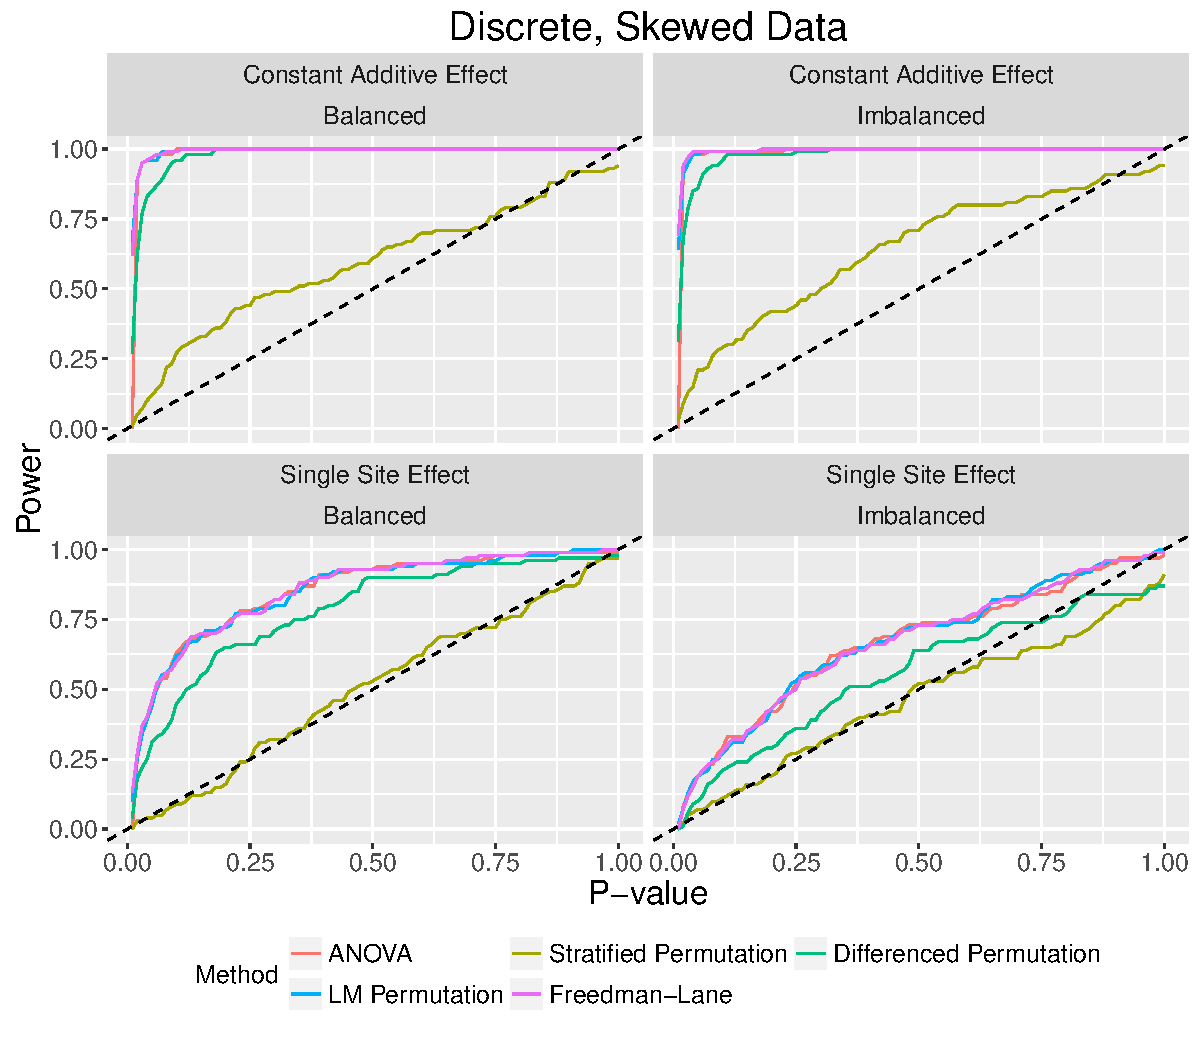
\includegraphics[width = \textwidth]{fig/skewed_simulation_power}
\caption{Empirical power curves for the skewed, discrete simulated data}
\label{fig:skewed_sim_power}
\end{figure}

\begin{center}
\begin{table}[ht]
\centering
\begin{tabular}{p{1.25in}|p{0.7in}|p{0.6in}p{0.8in}p{0.8in}p{0.8in}p{0.75in}}
  \hline
Treatment & Design & ANCOVA & Stratified Permutation & Differenced Permutation & LM Permutation & Freedman-Lane \\ 
  \hline
No Effect & Balanced & 0.036 & 0.025 & 0.021 & 0.035 & 0.037 \\ 
  Constant Additive Effect & Balanced & 0.974 & 0.143 & 0.853 & 0.972 & 0.977 \\ 
  Single Stratum Effect & Balanced & 0.422 & 0.050 & 0.275 & 0.429 & 0.424 \\ 
   \hline
No Effect & Imbalanced & 0.038 & 0.024 & 0.019 & 0.037 & 0.039 \\ 
  Constant Additive Effect & Imbalanced & 0.971 & 0.147 & 0.860 & 0.970 & 0.972 \\ 
  Single Stratum Effect & Imbalanced & 0.190 & 0.070 & 0.100 & 0.190 & 0.190 \\ 
   \hline
\end{tabular}
\caption{Empirical power at level $0.05$ for discrete, skewed simulated data} 
\label{tab:skewed_power}
\end{table}

\end{center}

It makes sense that in all of these simulations, the permutation test using the difference in outcome and baseline as the response measure is more powerful than the permutation test using the raw outcomes.
In additional simulations\footnote{see supplementary files on GitHub}, we changed the Gaussian model so that the outcome and baseline had correlation of $0.25$.
In this case, the result was reversed: the differenced test had low power while the test using the raw outcomes had a power curve closer to the tests that adjust for covariates using a linear model.
This phenomenon has been studied before \todo{cite}, and it is recommended to use the difference in outcome and baseline only when their correlation is larger than $0.5$ (\cite{frison_repeated_1992}).



\subsection{Clinical data results}

\bit
\item mention that we thought about whether to use the raw outcomes and adjust for baseline, or use outcome minus baseline. The outcome and baseline had a low correlation (include here), so we did not use their difference. As the simulations show, doing this actually reduces power
\item Freedman-Lane stuff: for the appro
For this dataset, we are guaranteed that treatment $Z$ is independent of $\varepsilon$, as it is randomized within site.
Indeed, the distribution of residuals looks nearly equal between treatment groups in both models.
The distribution of residuals varies a bit across sites, but they all appear roughly centered around 0.
Sites 4 and 5 have larger variance in the differenced model.
As mentioned, this should not be an issue since we permute treatments within sites, independently across sites.
(In general, when treatment is not randomly assigned, this condition is necessary for the permutation test to be valid.)
\eit

\begin{center}
\begin{table}[ht]
\centering
\begin{tabular}{r|p{1.2in}p{1.2in}p{1.2in}p{1.2in}}
  \hline
 & Parametric ANCOVA & Stratified permutation & LM permutation & Residual permutation \\ 
  \hline
heart\_freq & 0.035 & 0.006 & 0.080 & 0.082 \\ 
  regurg\_freq & 0.136 & 0.118 & 0.280 & 0.220 \\ 
  dysp\_freq & 0.565 & 0.948 & 0.616 & 0.592 \\ 
  daily\_heart & 0.032 & 0.004 & 0.056 & 0.068 \\ 
  daily\_regurg & 0.142 & 0.174 & 0.286 & 0.246 \\ 
  daily\_hrdq & 0.043 & 0.012 & 0.088 & 0.098 \\ 
  daily\_dysp & 0.582 & 0.810 & 0.756 & 0.722 \\ 
   \hline
\end{tabular}
\caption{Comparison of p-values from four tests, for each continuous endpoint.} 
\label{tab:clinical_pvalues}
\end{table}

\end{center}

\section{Discussion}
% This section should discuss the implications of the findings in context of existing research and highlight limitations of the study.

\bit
\item This paper adds to the literature comparing parametric and nonparametric tests
\item In randomized control trials, there is no substantial difference between parametric and nonparametric approaches.  They are asymptotically equivalent to begin with (find a citation). But our simulations, using small sample sizes, show that they give comparable results anyway.
\item Results about differenced vs raw outcomes. This isn't new but our simulations and empirical dataset confirm it in the context of permutation tests
\item 
\eit


% list of abbreviations

\section{Declarations}
% see http://bmcmedresmethodol.biomedcentral.com/submission-guidelines/preparing-your-manuscript/technical-advance-article
\textbf{Ethics approval and consent to participate}
Not applicable
\textbf{Consent for publication}
\textbf{Availability of data and material}
\textbf{Competing interests}
\textbf{Funding}
\textbf{Authors' contributions}
\textbf{Acknowledgements}
\textbf{Authors' information}

\bibliographystyle{plainnat}
\bibliography{references}




\end{document}